%!TEX root = ../Thesis.tex

\section{Feedforward Neural Network}

The models presented there are all neural networks or can be interpreted as such. To give a short introduction to neural networks and how they are constructed, used and trained the feedforward neural network (FFNN) is used. The feedforward neural network is properly the simplest model in the family of neural networks and the other models can be considered as extensions of the FFNN. An exception to this is perhaps the skip-gram model which may be slightly simpler.

\subsection{The neuron}

The neuron is the main construct in any neural network. Mathematically it is just a function which takes a vector and returns a scalar. It does this by a weighed linear combination of the inputs:
\begin{equation}
a = \sum_{i=1}^I w_{i} x_i
\end{equation}

This linear combination is then typically transformed using a non-linear function $\theta$:
\begin{equation}
b = \theta(a)
\end{equation}

The value $b$ is then the output of the neuron and is called the activation. Typically the sigmoid function $\sigma(\cdot)$ or hyperbolic tangent $\tanh(\cdot)$ function is used \cite{bishop}. If no non-linear function is applied then the identity function is used $\theta(a) = a$.

\begin{figure}[H]
	\centering
	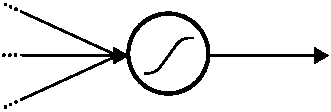
\includegraphics[scale=0.7]{theory/ffnn-neuron}
	\caption{Visual representation of a single neuron. The left arrows represents an input elements ($x_i$). The circle represent the function there returns a scalar (right arrow).}
\end{figure}

\subsection{The network}

A neural network is a multivariable non-linear regression model constructed by combining multiply neurons, but can be slightly expanded to become a multiclass classifier. This is done by using a the softmax function \cite{the-elements-of-statistical-learning}, such each output value is the class probability $y_k = P(C_k | x)$.

\begin{figure}[h]
	\centering
	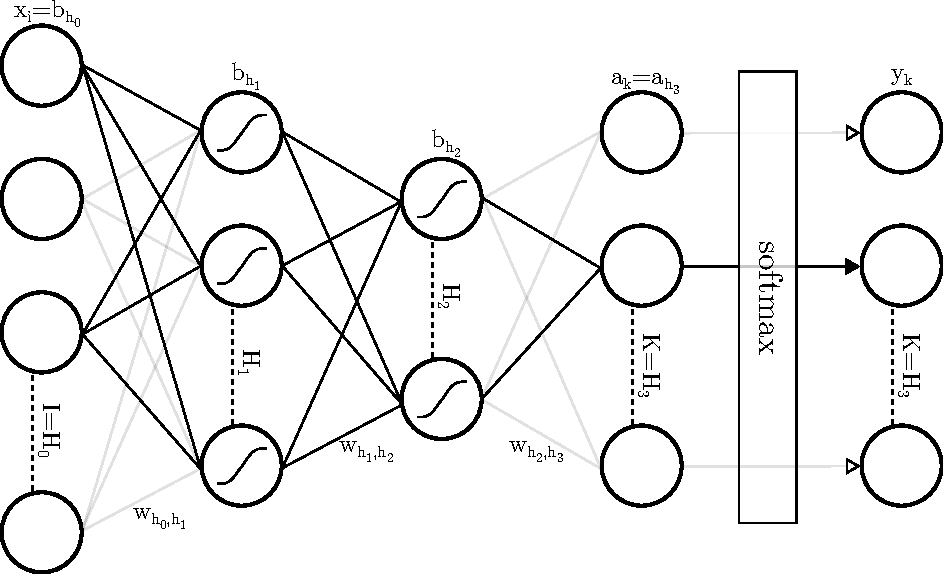
\includegraphics[scale=0.7]{theory/ffnn-network.pdf}
	\caption{Visual representation of a neural network with two hidden layers. Some lines are less visibel, this is just a visual aid because the many lines can be difficult to look at.}
	\label{fig:theory:ffnn:network}
\end{figure}

The neural network in Figure \ref{fig:theory:ffnn:network}, have one input layer $x_i, i \in [1, I]$ and one output layer $y_k, k \in [1, K]$. This is always the case for a neural network what varies is the type of network (here a feedforward neural network) and the amount of hidden layers (here two). The hidden layers are those layers there can contain non-linear functions. If there are no hidden layers, the neural network i just a multivariate linear regression or a multiclass logistic regression if the softmax is applied \cite{bishop}.

Because there are multiply neurons in each layer and multiply layers, the neuron index and layer is denoted by the subscript. For example a neuron output is denoted by $b_{h_{\ell}}$ for $h_{\ell} \in [1, H_{\ell}]$, where $h_{\ell}$ is the neuron index in layer $\ell$.

\subsection{Forward pass}

Calculation of the network output ($y_k$) is sometimes called the \textit{forward pass}, while the parameter estimation is sometimes called the \textit{backward pass}.

First the activation for the first layer is calculated:
\begin{equation}
\begin{aligned}
b_{h_1} = \theta(a_{h_1}), && a_{h_1} = \sum_{i = 1}^I w_{i, h_1} x_i, && \forall h_1 \in [1, H_1]
\end{aligned}
\end{equation}

The activation for the second layer is almost identical:
\begin{equation}
\begin{aligned}
b_{h_2} = \theta(a_{h_2}), && a_{h_2} = \sum_{h_1 = 1}^{H_1} w_{h_1, h_2} b_{h_1}, && \forall h_2 \in [1, H_2]
\end{aligned}
\end{equation}

In fact by letting $x_i = b_{h_0}$ the activation can be generalized to any amount of hidden layers ($L$):
\begin{equation}
\begin{aligned}
b_{h_\ell} &= \theta(a_{h_\ell}), && \forall h_{\ell} \in [1, H_{\ell}] \wedge \ell \in [1, L] \\
a_{h_\ell} &= \sum_{h_{\ell-1} = 1}^{H_{\ell-1}} w_{h_{\ell-1}, h_{\ell}} b_{h_{\ell-1}}, && \forall \ell \in [1, L+1] \text{ where: } b_{h_0} = x_i, H_0 = I \\
\end{aligned}
\end{equation}

At last the network output $y_k$ can be calculated using the softmax function on the $a_{L+1}$ results:
\begin{equation}
\begin{aligned}
y_k = \frac{\exp(a_k)}{\sum_{k'=1}^K \exp(a_{k'})}, && \forall k \in [1, K] \text{ where: } a_k=a_{h_{L+1}}, K = H_{L + 1}
\end{aligned}
\label{eq:theory:ffnn:y}
\end{equation}

\subsection{Loss function}

Optimization of the parameters $w_{i,j}$ requires definition of a loss function. For classification it makes sense to maximize the joint probability of observing all the observations:
\begin{equation}
P(\mathbf{t} | \mathbf{x}, \mathbf{w}) = \prod_{n=1}^N P(\mathbf{t}_n | \mathbf{x}_n, \mathbf{w})  = \prod_{n=1}^N \prod_{k=1}^K P(C_{n, k} | \mathbf{x}_n, \mathbf{w})^{t_{n, k}}
\end{equation}

Here $\mathbf{x}_{n}$ is the input vector for observation $n$, with a corresponding label vector $\mathbf{t}_n$. The label vector is an indicator vector, constructed such using 1-of-K encoding. For example if there are 5 classes and, class 2 is the correct class for observation $n$, then $\mathbf{t}_n = [0, 1, 0, 0, 0]^T$.

The negative logarithm is then used to create linearity and avoid floating point errors:
\begin{equation}
- \ln\left(P(\mathbf{t} | \mathbf{x}, \mathbf{w})\right) = - \sum_{n=1}^N \sum_{k=1}^K t_{n, k} \ln\left( P(C_{n, k} | \mathbf{x}_n, \mathbf{w})\right)
\end{equation}

Because all the following uses of this loss function isn't influenced by the sum over $n$, the $n$ index is typically omitted. The loss function will also be denoted by $\mathcal{L}$:
\begin{equation}
\mathcal{L} = - \sum_{k=1}^K t_{k} \ln\left( P(C_{k} | \mathbf{x}, \mathbf{w})\right) =  - \sum_{k=1}^K t_k \ln(y_k)
\label{eq:theory:ffnn:loss}
\end{equation}

\subsection{Backward pass}

For the neural network there is no closed form solution to the loss function, thus an iterative algorithm called gradient decent is used. Gradient decent uses the derivatives of the loss function with respect to the parameters to iteratively optimize the parameters. This approach will be discussed in details later, for now the important part is to find a method of calculating the derivatives.

For calculating the derivatives the \textit{error backprobagation} algorithm is used. The name varies a bit depending on the neural network architecture (in this case feedforward), thus the term \textit{backward pass} will be used as the umbrella term.

The neural network from earlier in Figure \ref{fig:theory:ffnn:network} will be used to inspire the general algorithm. The overall goal is to calculate:
\begin{equation}
\begin{aligned}
\frac{\partial \mathcal{L}}{\partial w_{h_{\ell-1}, h_\ell}}, && \forall \ell \in [1, L + 1]
\end{aligned}
\label{eq:theory:ffnn:bprop-problem}
\end{equation} 

First consider the problem in \eqref{eq:theory:ffnn:bprop-problem} for the layer $\ell = 1$. This will depend on some hidden input $a_{h_1}$ in the first hidden layer, thus the chain rule can be used:
\begin{equation}
\frac{\partial \mathcal{L}}{\partial w_{h_0, h_1}} = \frac{\partial \mathcal{L}}{\partial a_{h_1}} \frac{\partial a_{h_1}}{\partial w_{h_0, h_1}} =  \frac{\partial \mathcal{L}}{\partial a_{h_1}} x_{h_0}
\label{eq:theory:ffnn:bprop-firstlayer}
\end{equation}

It turns out that it is smart to define $\frac{\partial \mathcal{L}}{a_{h_1}}$ in general for all layers, this is just a form of book keeping there will make it easier to implement.
\begin{equation}
\delta_{h_\ell} \defeq \frac{\partial \mathcal{L}}{\partial a_{h_\ell}}
\end{equation}

Using this \eqref{eq:theory:ffnn:bprop-firstlayer} becomes:
\begin{equation}
\frac{\partial \mathcal{L}}{\partial w_{h_0, h_1}} = \delta_{h_1} x_{h_0}
\label{eq:theory:ffnn:bprop-w01}
\end{equation}

The equation ``how should $\delta_{h_1}$ be calculated ?'' then arises. This is done by using the chain rule again. This time the chain rule gives a sum because there are multiply paths $a_{h_1}$. \todo{I don't fully understand this}
\begin{equation}
\delta_{h_1} = \frac{\partial \mathcal{L}}{\partial a_{h_1}} = \sum_{h_2=1}^{H_2} \frac{\partial \mathcal{L}}{\partial a_{h_2}} \frac{\partial a_{h_2}}{\partial a_{h_1}}
\end{equation}

A chain rule is then again used, this time for expanding $\frac{\partial a_{h_2}}{\partial a_{h_1}}$:
\begin{equation}
\begin{aligned}
\delta_{h_1}
&= \frac{\partial \mathcal{L}}{\partial a_{h_1}}
= \sum_{h_2=1}^{H_2} \frac{\partial \mathcal{L}}{\partial a_{h_2}} \frac{\partial a_{h_2}}{\partial b_{h_1}} \frac{\partial b_{h_1}}{\partial a_{h_1}}
= \frac{\partial b_{h_1}}{\partial a_{h_1}} \sum_{h_2=1}^{H_2} \frac{\partial \mathcal{L}}{\partial a_{h_2}} \frac{\partial a_{h_2}}{\partial b_{h_1}} \\
&= \theta'(a_{h_1}) \sum_{h_2=1}^{H_2} \delta_{h_2} w_{h_1, h_2}
\end{aligned}
\label{eq:theory:ffnn:bprop-secondlayer}
\end{equation}

Calculating $\delta_{h_2}$ is almost identical:
\begin{equation}
\begin{aligned}
\delta_{h_2}
&= \frac{\partial \mathcal{L}}{\partial a_{h_2}}
= \sum_{h_3=1}^{H_3} \frac{\partial \mathcal{L}}{\partial a_{h_3}} \frac{\partial a_{h_3}}{\partial b_{h_2}} \frac{\partial b_{h_2}}{\partial a_{h_2}}
= \frac{\partial b_{h_2}}{\partial a_{h_2}} \sum_{h_3=1}^{H_3} \frac{\partial \mathcal{L}}{\partial a_{h_3}} \frac{\partial a_{h_3}}{\partial b_{h_2}} \\
&= \theta'(a_{h_2}) \sum_{h_3=1}^{H_3} \delta_{h_3} w_{h_2, h_3}
\end{aligned}
\label{eq:theory:ffnn:bprop-thirdlayer}
\end{equation}

Calculating $\delta_{h_3}$ will be a bit different, because it is the last $\delta_{h_\ell}$ there needs calculation (for a neural network with two hidden layer). It thus makes sense first to generalize \eqref{eq:theory:ffnn:bprop-secondlayer} and \eqref{eq:theory:ffnn:bprop-thirdlayer} such that it can work for any number of hidden layers:
\begin{equation}
\begin{aligned}
\delta_{h_\ell} = \theta'(a_{h_\ell}) \sum_{h_\ell=1}^{H_\ell} \delta_{h_\ell} w_{h_{\ell-1}, h_\ell}, && \forall \ell \in [1, L]
\end{aligned}
\label{eq:theory:ffnn:bprop-genalized}
\end{equation}

The last delta $\delta_{h_3}$ or in general $\delta_{h_{L+1}}$ is calculated by using a chain rule on the $y_k$ variables. This is because $y_k$ are the only variables between $a_{L+1}$ and $\mathcal{L}$:
\begin{equation}
\delta_{h_{L + 1}} = \delta_k = \frac{\partial \mathcal{L}}{\partial a_k} = \sum_{k'=1}^K \frac{\partial \mathcal{L}}{\partial y_{k'}} \frac{\partial y_{k'}}{\partial a_k}
\label{eq:theory:ffnn:bprop-deltaK}
\end{equation}

The first partial derivatives can be derived from \eqref{eq:theory:ffnn:loss}:
\begin{equation}
\frac{\partial \mathcal{L}}{\partial y_{k'}} = \frac{\partial}{\partial y_{k'}} \left(- \sum_{k''=1}^K t_{k''} \ln(y_{k''})\right) = -\frac{t_{k'}}{y_{k'}}
\label{eq:theory:ffnn:bprop-Ldy}
\end{equation}

The other partial derivatives can be derived from \eqref{eq:theory:ffnn:y}:
\begin{equation}
\begin{aligned}
\frac{\partial y_{k'}}{\partial a_k}
&= \frac{\partial}{\partial a_k} \frac{\exp(a_{k'})}{\sum_{k''=1}^K \exp(a_{k''})} \\
&= \frac{\frac{\partial}{\partial a_k} \exp(a_{k'})}{\sum_{k''=1}^K \exp(a_{k''})}
- \frac{\exp(a_{k'}) \frac{\partial}{\partial a_k} \sum_{k''=1}^K \exp(a_{k''})}{\left(\sum_{k''=1}^K \exp(a_{k''})\right)^2} \\
&= \frac{\frac{\partial}{\partial a_k} \exp(a_{k'})}{\sum_{k''=1}^K \exp(a_{k''})}
- \frac{\exp(a_{k'})}{\sum_{k''=1}^K \exp(a_{k''})} \frac{\frac{\partial}{\partial a_k} \sum_{k''=1}^K \exp(a_{k''})}{\sum_{k''=1}^K \exp(a_{k''})}
\end{aligned}
\end{equation}

Because of the difference in index the first term is only not zero when $k = k'$, in which case $y_k$ is the result. It thus becomes useful to define:
\begin{equation}
\delta_{i,j} = \begin{cases}1& \text{when } i = j \\ 0 & \text{otherwise}\end{cases}
\end{equation}

The partial derivative in the second term is $\exp(a_k)$, because $\frac{\partial}{\partial a_k} \exp(a_{k''})$ is zero except in the case where $k = k''$.
\begin{equation}
\frac{\partial y_{k'}}{\partial a_k} = \delta_{k, k'} y_k - y_{k'} y_k
\label{eq:theory:ffnn:bprop-yda}
\end{equation}

The result from \eqref{eq:theory:ffnn:bprop-Ldy} and \eqref{eq:theory:ffnn:bprop-yda} is then combined intro \eqref{eq:theory:ffnn:bprop-deltaK}:
\begin{equation}
\begin{aligned}
\delta_{h_{L + 1}} = \delta_k &= \sum_{k'=1}^K -\frac{t_{k'}}{y_{k'}} \left( \delta_{k, k'} y_k - y_{k'} y_k \right) = \sum_{k'=1}^K -\frac{t_{k'}}{y_{k'}} \delta_{k, k'} y_k + \sum_{k'=1}^K \frac{t_{k'}}{y_{k'}} y_{k'} y_k \\
&= -\frac{t_k}{y_k} y_k + y_k \sum_{k'=1}^K t_{k'} = -t_k + y_k = y_k - t_k
\end{aligned}
\label{eq:theory:ffnn:bprop-deltaKfinal}
\end{equation}

In the last step it was used that $\{ t_{k'} \}_{k'=1}^K$ is constructed using 1-of-K encoding, thus only one element is 1 and the remaining is 0. A sum of all elements must therefore give 1.

Using \eqref{eq:theory:ffnn:bprop-deltaKfinal} and \eqref{eq:theory:ffnn:bprop-genalized} all $\delta_{h_\ell}$ for $\ell \in [1, L+1]$ can be calculated for a feedforward neural network with $L$ layers. Note how \eqref{eq:theory:ffnn:bprop-deltaKfinal} is an error and this error is propagated back though the network by the $\delta_{h_\ell}$ equations in \eqref{eq:theory:ffnn:bprop-genalized}. This is why the method is called \textit{error backpropagation}.

Given the $\delta_{h_1}$ the weights $w_{h_0, h_1}$ can be calculated using \eqref{eq:theory:ffnn:bprop-w01}. However the weights $w_{h_0, h_1}$ are not the only parameters. Luckily the equations for the other $w_{h_{\ell-1}, h_\ell}$ are not much different.
\begin{equation}
\begin{aligned}
\frac{\partial \mathcal{L}}{\partial w_{h_{\ell-1}, h_\ell}} = \frac{\partial \mathcal{L}}{\partial a_{h_\ell}}
\frac{\partial a_{h_\ell}}{w_{h_{\ell-1}, h_\ell}} = \delta_{h_\ell} b_{h_{\ell-1}}, && \forall \ell \in [1, L+1] \text{ where: } b_{h_0} = x_i
\end{aligned}
\end{equation}

\todo{Consider formalizing a vector notation of the forward and backward pass.}
